\section{Empirical Risk Minimization}
\begin{definition}[Generalization \& Empirical Error]
	\begin{align}
		(\text{Generalization}) \quad & \cR(\widehat{c}) = p(\widehat{c}(\bfx) \neq c(\bfx)) \\
		(\text{Empirical}) \quad & \widehat{\cR}(\widehat{c}) = \frac{1}{n} \sum_i \Ind{c(\bfx_i) \neq y_i}
	\end{align}
\end{definition}
\begin{definition}[ERM]
 Empirical Risk Minimization (ERM) means selecting the classifier $\widehat{c}_n \in \cC $ with the smallest error on the training data $Z = \{(\bfx_1. y_1), \cdots, (\bfx_n. y_n) \}$, i,e,,
 $$
 \widehat{c}_n = \argmin_{c \in \cC} \widehat{\cR}_n(c), \where \widehat{\cR}_n(c) = \frac{1}{n} \sum_i \Ind{c(\bfx_i) \neq y_i}.
 $$
 Here, $\widehat{\cR}_n(c)$ is called the \textbf{empirical error} of $c$.
\end{definition}


\begin{theorem}[Vapnik \& Chervonenkis] Let $c^* = \argmin_c \cR(c)$,
$$
\cR(\widehat{c}^*_n) - \inf_{c \in \cC} \cR(c) \leq 2 \sup_{c \in \cC} |\widehat{\cR}_n(c) - \cR_n(c) |.
$$
\end{theorem}
\begin{proof}
	\begin{align}
		\cR(\widehat{c}^*_n) - \inf_{c \in \cC} \cR(c) & = \cR(\widehat{c}^*_n) - \widehat{\cR}(\widehat{c}^*_n) + \widehat{\cR}(\widehat{c}^*_n) - \inf_{c \in \cC} \cR(c)\\
		& \leq \cR(\widehat{c}^*_n) - \widehat{\cR}(\widehat{c}^*_n) + \widehat{\cR}({c}^*_n) - \cR({c}^*) \\
		& \leq \sup_{c \in \cC} | \cR(c) - \widehat{\cR}(c) | + \sup_{c \in \cC} | \widehat{\cR}(c) - \cR(c)| \\
		& \leq 2 \sup_{c \in \cC} | \cR(c) - \widehat{\cR}(c) |.
	\end{align}
\end{proof}

\section{PAC Learning Model}
A learning algorithm $\cA$ can learn a concept class $\cC$ from $\cH$ if, given as input a sufficiently large sample, it outputs a hypothesis that generalizes well with high probability.
\begin{definition}[PCA Learnable]
	A learning algorithm $\cA$ can learn a concept class $\widehat{c}^*_n \in \cC$ from $\cH$, if there is a polynomial function $\mathrm{poly}(\cdot, \cdot, \cdot)$ such that: (1) for any distribution $\cD$ on $\cX \times \{0, 1\}$ and (2) for any $0 < \epsilon < 1/2$, $0 < \delta < 1/2$,
\begin{equation}
	p_{Z \sim \cD^n}\left( \cR(\widehat{c}^*_n) - \inf_{c \in \cC} \cR(c) \leq \epsilon \right) \geq 1 - \delta, \where n \geq \mathrm{poly}(1/\epsilon, 1/\delta, dim(\cX)).
\end{equation}
Here, $\cD^n$ means the training set of $n$ samples, i.e., $\cD^n = \{(\bfx_1, y_1), \cdots,  (\bfx_n, y_n)\}$.
\end{definition}
\begin{property}[Universal Concept Class]
	Universal concept class is not PAC learnable. Let $\cX = \{0, 1\}^*$ be the set of all finite binary sequences. The concept class $\cC$ formed by all subsets of $\cX$ is not PAC learnable from $C$.
\end{property}

\begin{definition}[Efficient PAC Learning]
	If $\cA$ runs in \textbf{polynomial} time in $1/\epsilon$ and $1/\delta$, we say that $\cA$ is an  efficient PAC learning algorithm.
\end{definition}

\subsection{Finite Hypothesis Classes}
In this section, we assume that the hypothesis class is finite.  Let $|\cH|$ denote the cardinality of $\cH$.
\begin{theorem}[Error Bound - Consistent Hypothesis Classes]
	Let $\cC$ be a finite concept class, $\cH$ be a consistent hypothesis class  $\cH = \cC$ and $\cA$ be an algorithm that returns a consistent hypothesis $\widehat{c}$ (i.e., $\forall n < \infty: \widehat{\cR}_n(\widehat{c}) = 0$).
	
	For any target concept $c \in \cC$ and any i.i.d. sample $Z$, for any $\epsilon > 0$, there exists $\delta > 0$ such that
	\begin{equation}
		p_{}({\cR}(\widehat{c}) \leq \epsilon) \geq 1 - \delta, \where n \geq \frac{1}{\epsilon}\left( \log |\cH| + \log \frac{1}{\delta} \right).
	\end{equation}
\end{theorem}
\begin{proof}
In consistent case, we have assumed that the empirical error $\widehat{\cR}_n(\widehat{c}) = 0$.
\begin{align}
	p\left( \sup_{c \in \cC} {\cR}(\widehat{c}) > \epsilon \right) & \leq \sum_{c \in \cC}  p\left( {\cR}(\widehat{c}) > \epsilon  \cap \widehat{\cR}_n(\widehat{c}) = 0 \right) \\
	& \leq \sum_{c \in \cC}  p\left( \widehat{\cR}_n(\widehat{c}) = 0 \mid {\cR}(\widehat{c}) > \epsilon \right) \\
	& \leq |\cH| (1 - \epsilon)^n
\end{align}
Then, we can solve the $n$ from this inequality, which brings us to the conclusion.
\end{proof}


\begin{theorem}[Error Bound - Inconsistent Hypothesis Classes]
	Let $\cC$ be a finite concept class, $\cH$ be a inconsistent hypothesis class  $\cH \neq \cC$ and $\cA$ be an algorithm that returns a consistent hypothesis $\widehat{c}$ (i.e., $\forall n < \infty: \widehat{\cR}_n(\widehat{c}) = 0$).
	
	For any target concept $c \in \cC$ and any i.i.d. sample $Z$, for any $\epsilon > 0$, there exists $\delta > 0$ such that
	\begin{equation}
		p_{}\left(\sup_{c \in \cC} |\widehat{\cR}_n(\widehat{c}) - {\cR}(\widehat{c}) | \leq \epsilon \right) \geq 1 - \delta, \where n \geq \frac{1}{2\epsilon^2}\left( \log |\cH| + \log \frac{2}{\delta} \right).
	\end{equation}
\end{theorem}
\begin{proof}
	Using the Hoeffding inequality, we have
	\begin{align}
		p_{}\left(\sup_{c \in \cC} |\widehat{\cR}_n(\widehat{c}) - {\cR}(\widehat{c}) | \leq \epsilon \right) & \leq \sum_{c \in \cC} p_{}\left(|\widehat{\cR}_n(\widehat{c}) - {\cR}(\widehat{c}) | \leq \epsilon \right) \\
		& \leq 2 |\cH| \exp(-2 n \epsilon^2 )
	\end{align} 
Then, we can solve the $n$ from this inequality, which brings us to the conclusion.
\end{proof}
\remark This theorem can be also written into the following form. The variance depends on sample size as $1/\sqrt{n}$, but only logarithmically on the size of the hypothesis class as $\log |\cH|$ .
\begin{align}
	\underbrace{{\cR}(\widehat{c})}_\text{expected error} \leq \underbrace{\widehat{\cR}_n(\widehat{c})}_\text{empirical error} + \underbrace{\sqrt{\frac{\log |\cH| + \log \frac{2}{\delta}}{2n}}}_\text{variance},\quad \forall c \in \cC.
\end{align}
\subsection{Example: Learning Axis-aligned Rectangles}
Let $\cC$ be the concept of all axis-aligned rectangles $R$. We show that $\cC$ can be learned from $\cH = \cC$. 
\begin{figure}[h]
\center
	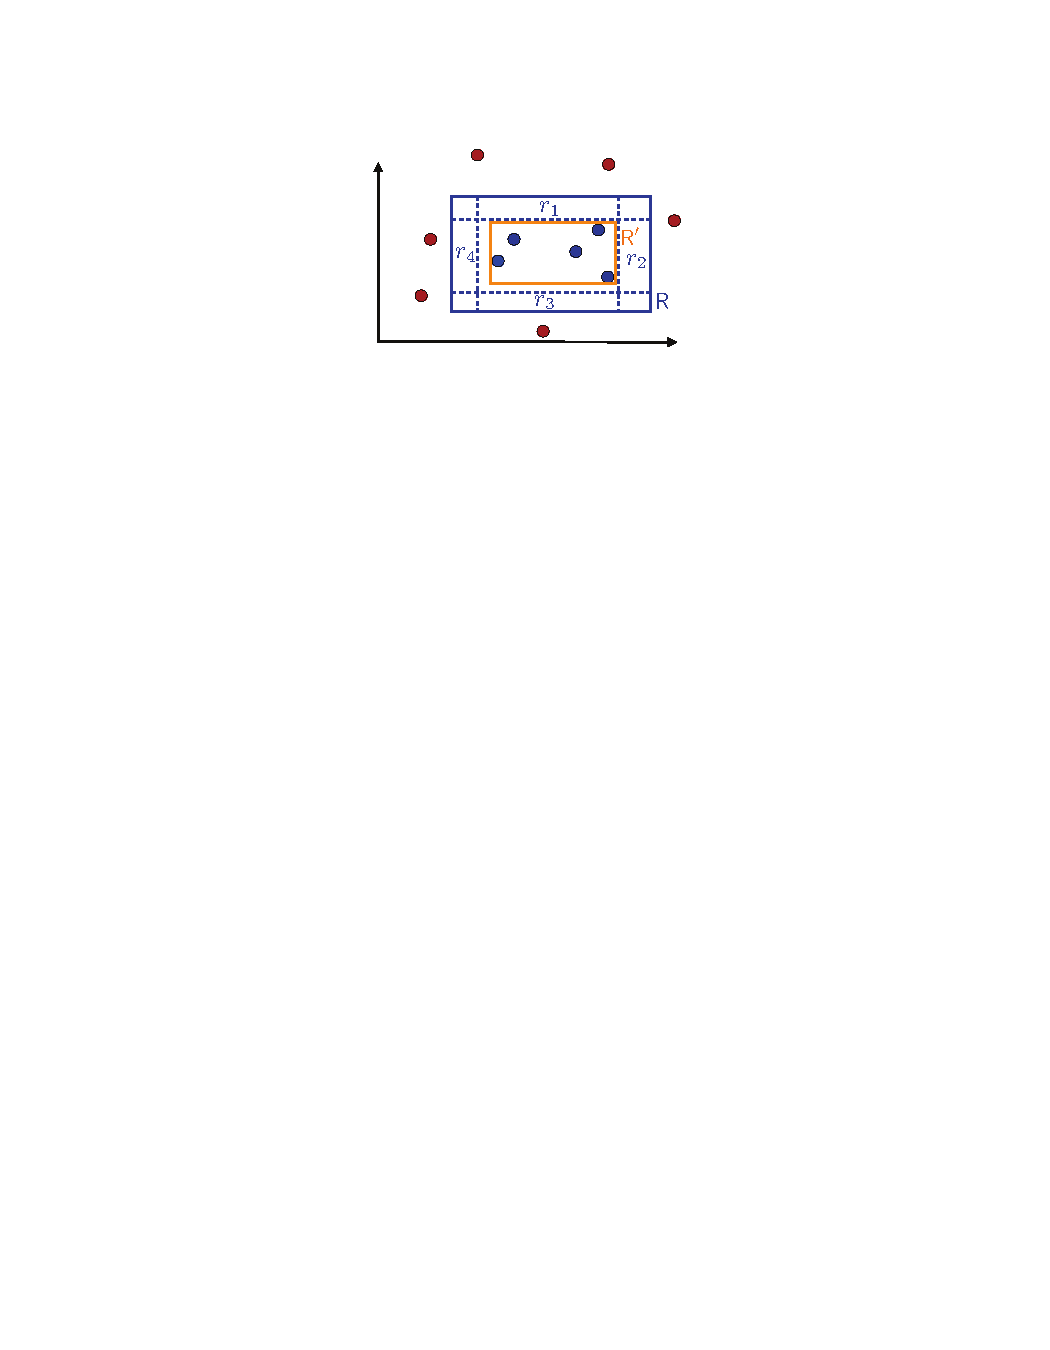
\includegraphics[width=0.5\linewidth]{figures/PAC_rect}
	\caption{Illustration of rectangle $R$ and ``RIG'' regions. \label{fig:pca}}
\end{figure}

See Fig.~\ref{fig:pca}, consider the algorithm $\cA$ finds the smallest rectangle $R'$ containing all positive points. \footnote{This figure is taken from M. Mohri, Foundations of Machine Learning, 2018} We will show that $\cA$ can learn any concept of $R \in \cC$.
\begin{theorem}[Axis-aligned Rectangles are PCA Learnable] Given a dataset with $n$ points, for any $\delta > 0, \epsilon > 0$, to ensure that $p(\cR(R') > \epsilon) \leq \delta$, we can impose a constraint that
$$
 n \geq \mathrm{poly}(1/\epsilon, 1/\delta, \mathrm{size}(R')=4) = \frac{4}{\epsilon} \log \frac{4}{\delta}.
$$
\end{theorem}
\begin{proof}
	Given a prediction $R'$, its risk $\cR(R')$ is the sum of probability of false negative and false positive. More precisely,
	\begin{equation}
		\cR(R') = p\left( \underbrace{(R - R')}_{\text{false neg.}}\ \cup\ \underbrace{(R' - R)}_{false pos.} \right) = p(R - R').
	\end{equation}
	We define four stripes of the $R$, $r_1, r_2, r_3, r_4$, as shown in Fig.~\ref{fig:pca}. Each of the stripe has probability at least $\epsilon / 4$. If the risk exceed $\epsilon$, then $R'$ does not hit at least one of the stripes. We can write,
	\begin{align}
		p(\cR(R') \geq \epsilon) & \leq p_D\left(\bigcup_{i \leq 4} R' \cap r_i = \emptyset\right) \\
		& \leq \sum_{i \leq 4} p_D(R' \cap r_i = \emptyset) \\
		& \leq 4 (1 - \epsilon / 4)^n \\
		& \leq 4 \exp{(-n \epsilon / 4 )}. \qquad\qquad  (1 - x \leq e^{-x})
	\end{align}
To ensure $p(\cR(R') \geq \epsilon) \leq \delta$, we have
\begin{equation}
	4 \exp{(-n \epsilon / 4 )} \leq \delta \ \Longleftrightarrow \ n \geq \frac{4}{\epsilon} \log \frac{4}{\delta}
\end{equation}
\end{proof}             

\section{VC Dimension}
In Vapnik–Chervonenkis theory, the Vapnik–Chervonenkis (VC) dimension is a measure of the capacity (complexity) of a set of functions that can be learned by a \textbf{binary} classification algorithm. 
\begin{definition}
	VC dimension of $\cH$ is defined as the cardinality of the largest set of points on $\cH$ that the algorithm can shatter.
\end{definition}

\begin{table}[h]
{\setstretch{1.25}
\caption{Some interesting examples of VC dimension.}
\begin{tabular}{p{5.8cm} p{6.5cm} p{1.4cm}}
\toprule
	\textbf{Classifier} &  & \textbf{VC-dim} \\
	\midrule
stump classifier & $(-\infty, a]$, $a \in \R$  & $1$   \\
all intervals in $\R$ & $\{[a, b] \mid a, b \in \R \}$  & $2$   \\
all unions of $k$ intervals in $\R$  & $\{\bigcup_{i=1}^k [a_i, b_i] \mid a_i, b_i \in \R \}$ & $2k$  \\
all half-planes in $\R^2$ & $\{(x, y) \mid ax + by + c \geq 0, a, b, c \in \R \}$ & $3$  \\
all convex polygons in $\R^2$ & - & $\infty$ \\
all convex polygons with at most $k$ vertices in $\R^2$ & - & $2k + 1$ \\
\bottomrule
\end{tabular}
}
\end{table}


\section{Concentration Inequalities}
\begin{theorem}[Markov Inequality] Let $X$ be a non-negative random variable. Then
\begin{equation}
	p(X \geq \epsilon) \leq \frac{\EE[X]}{\epsilon}
\end{equation}
\end{theorem}
\begin{theorem}[Hoeffding inequality]
Let $X_1 , . . . , X_m$ be independent random variables with $X_i$ taking values in $[a_i, b_i]$ for all $i \in [m]$. Then, for any $\epsilon > 0$, the following inequalities hold for $S_m = \sum_{i=1}^m X_i$:
\begin{align}
	p(S_m - \EE[S_m] \geq \epsilon) \leq \exp\left( \frac{-2\epsilon^2}{\sum_{i=1}^m (b_i - a_i)^2} \right) \\
	p(S_m - \EE[S_m] \leq -\epsilon) \leq \exp\left( \frac{-2\epsilon^2}{\sum_{i=1}^m (b_i - a_i)^2} \right) 
\end{align}
\end{theorem}

\begin{theorem}[McDiarmid inequality]
Let $X_1, \cdots , X_m \in \mathcal{X}^m$ be a set of $m \geq 1$ independent random variables and assume that there exist $c_1 , \cdots , c_m > 0$ such that $f : \mathcal{X}^m \rightarrow \R$ satisfies the following conditions:	
$$|f(x_1,...,x_i,...,x_m) - f(x_1,...,x'_i,...x_m)|\leq c_i, $$
for all $i \in [m]$ and any points $x_1,...,x_m, x'_i \in \mathcal{X}$. Let $f(S)$ denote $f(X_1,...,X_m)$, then, for all $\epsilon > 0$, the following inequalities hold:
\begin{align}
	p(f(S) - \EE[f(S)] \geq \epsilon) \leq \exp\left( \frac{-2\epsilon^2}{\sum_{i=1}^m c_i^2} \right) \\
	p(f(S) - \EE[f(S)] \leq -\epsilon) \leq \exp\left( \frac{-2\epsilon^2}{\sum_{i=1}^m  c_i^2} \right) 
\end{align}
\end{theorem}
Note that \textit{Hoeffding inequality} is a special instance of \textit{McDiarmid inequality} where $f$ is defined by $f(S) = \frac{1}{m}\sum_{i=1}^m x_i$.
                                                                                                                                                                                                                                                                                                                                                                                                                                                                                                                                  
                                                                                                                                                                                                                                                                                                                                                                                                                                                                                                                                                                                                                                                                                                                                                                                                                                                                                                                                                                                                                                                                                                                                                                                                                                                                                                                                                                                    